\section{Application of Knots}
\begin{frame}{Alternating Knots}
 In these types of knots, if you follow any strand in any direction you switch between upside and downside at any crossing.
\begin{figure}
    \centering
    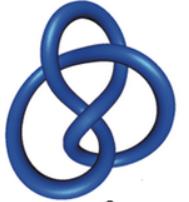
\includegraphics[height = 3.5cm, width= 8cm]{images/realalterknot.png}
    \caption{An alternating knot}
    \label{alterknot}
\end{figure}
\cite{https://doi.org/10.1002/anie.201702531}
\end{frame}
\begin{frame}{Rational Knots}
Rational knots are obtained by closing off the edges of rational tangles. A tangle is a region in a knot that is separated from the knot by a circle and has four outgoing strands crossing the circle. 
\begin{figure}[h]
    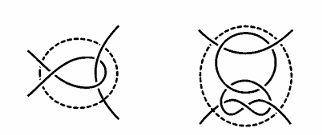
\includegraphics[width=0.6\linewidth]{images/tangles.png}
    \caption{Tangles}
    \label{tangles}
\cite{adams2004knot}
\end{figure}
\end{frame}
\begin{frame}
\begin{columns}[T]
\begin{column}{.48\textwidth}
\begin{figure}
    \centering
    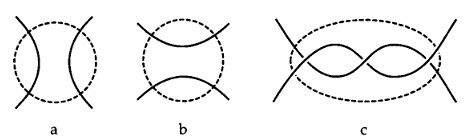
\includegraphics[width=0.9\linewidth,height=4cm]{images/basictangles.png}
    \caption{$\infty$, 0 and 3 tangles, they are \centering fundamental}
    \label{basictangles}
\end{figure}
\cite{adams2004knot}
\end{column}
\begin{column}{.48\textwidth}
\begin{figure}[h]
    \centering
    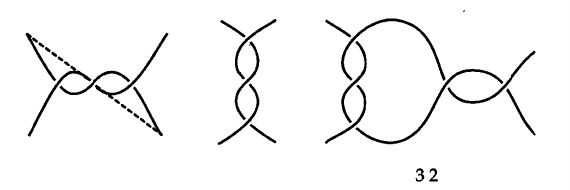
\includegraphics[width=0.9\linewidth,height=4cm]{images/tangleproduce.png}
    \caption{Generating Tangles}
    \label{generating}
\end{figure}
\end{column}
\end{columns}
\end{frame}
\begin{frame}{Pretzel Knots}
Pretzel knots are rational knots that are obtained by adding up rational tangles. If every term of a rational knot klm (for instant 311) is multiplied with 0 and then added altogether, the result is a pretzel knot that is denoted by k,l,m (3,1,1)
\begin{figure}
    \centering
    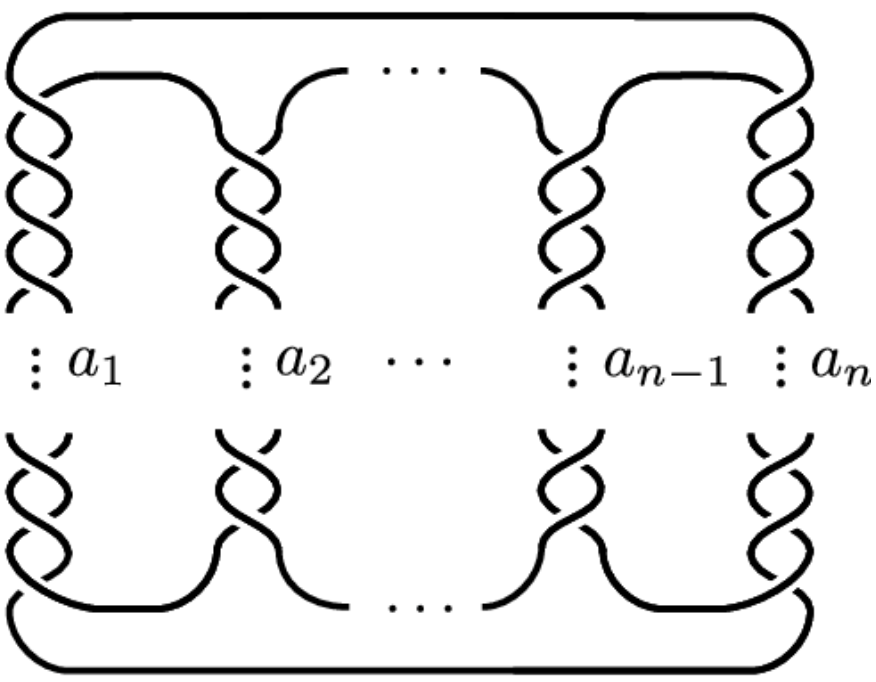
\includegraphics[width=0.4\linewidth]{images/pretzel.png}
    \label{pretzel}
    \cite{article2}
\end{figure}
\end{frame}
\begin{frame}{Torus Knots}
These knots are wrapped around unknotted tori and do not cross themselves as they move around their tori. There are 'short' paths called meridian and 'long' paths called longitude. A (p,q)-torus knot travels the longitude p times and travels meridians q times.
\begin{figure}
    \centering
    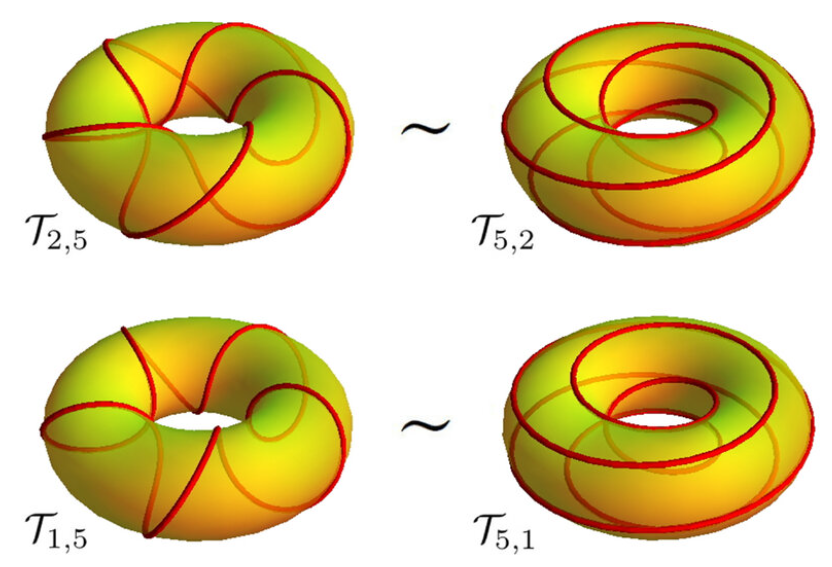
\includegraphics[height= 4cm, width=8cm]{images/torus.png}
    \label{torus}
   
\end{figure}
\cite{article}    
\end{frame}
\begin{frame}{Knots and Biology}
\begin{columns}[T]
\begin{column}{.48\textwidth}
\cite{555w}
\begin{figure}
    \centering
    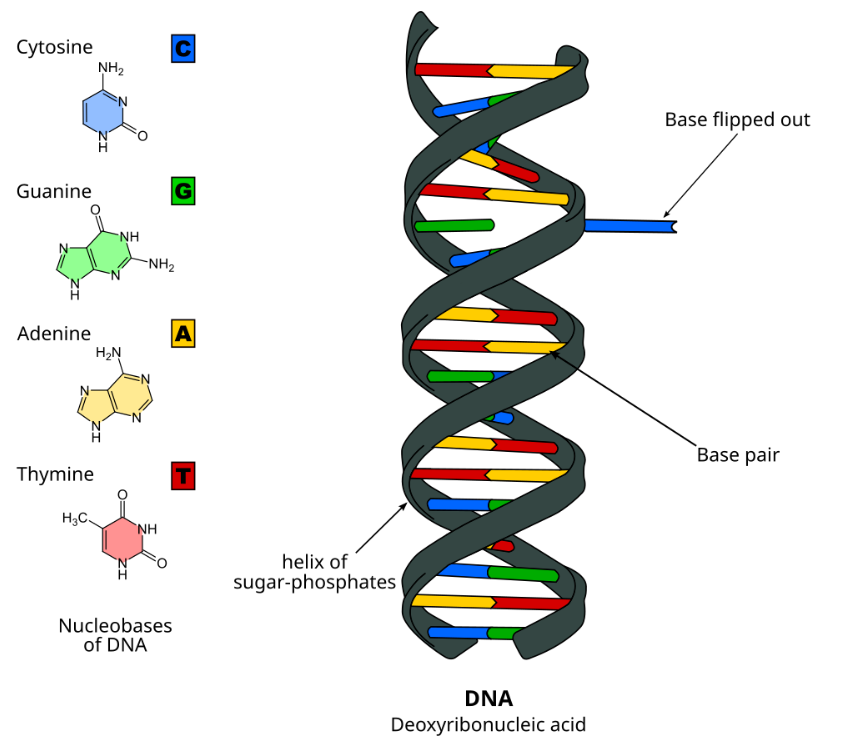
\includegraphics[width= 6cm,height=5.5cm]{images/dnastring.png}
    \label{dnast}
\end{figure}
\end{column}
\begin{column}{.48\textwidth}
\cite{adams2004knot}
\begin{figure}[h]
    \centering
    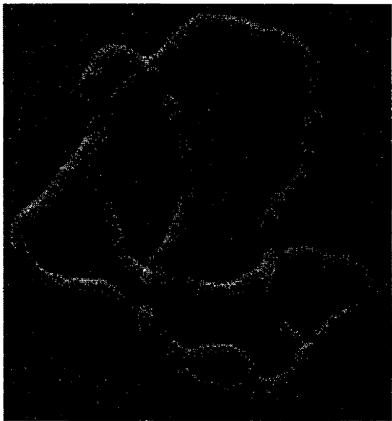
\includegraphics[width= 6cm,height=5.5cm]{images/electron.png}
    \label{elec}
\end{figure}
\end{column}
\end{columns}
\end{frame}
\begin{frame}
\begin{columns}[T]
\begin{column}{.48\textwidth}
\begin{itemize}
    \item \bold{Tw(R)}: Twist of the ribbon. Average of crossings over the axis
    \item \bold{Wr(R)}: Writhe of the ribbon. Average of crossings of the axis from every projection it is \\ \vspace{0.2cm} $\frac{\int signed-crossover-number.dA }{\int dA}$
    \item \bold{Lk(R)}: Linking number
    \item \bold{Lk(R) = Tw(R) + Wr(R)}
\end{itemize}
\end{column}
\begin{column}{.48\textwidth}
\begin{figure}
    \centering
    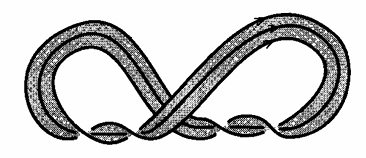
\includegraphics[width=0.6\linewidth]{images/ribbon.png}
    \caption{Axis}
    \label{axis}
    \cite{adams2004knot}
\end{figure}
\begin{figure}
    \centering
    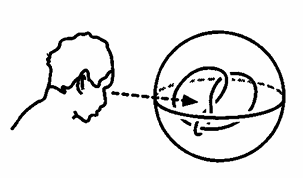
\includegraphics[width=0.6\linewidth]{images/vantage.png}
    \label{vantage}
    \cite{adams2004knot}
\end{figure}
\end{column}
\end{columns}
    
\end{frame}
\begin{frame}
\begin{columns}[T]
\begin{column}{.48\textwidth}
\begin{itemize}
\item S: Substrat tangle
\item T: Site tangle
\item R: Recombination tangle
\item N(Q): Converting tangle to a knot or a link
\item N(S + T) = N(1) (unknot)
\item N(S + R) = N(2) (Hopf link)
\item N(S + R + R) = N(211) (figure-eight knot)
\item N(S + R + R + R) = N(11111) (Whitehead link)
\end{itemize}
\end{column}
\begin{column}{.48\textwidth}
\begin{figure}
    \centering
    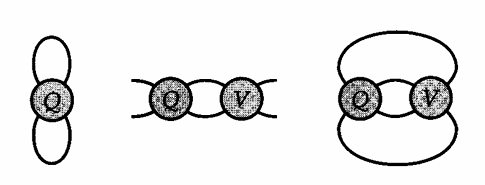
\includegraphics[width=1\linewidth]{images/subtang.png}
    \label{subtang}
    \cite{adams2004knot}
\end{figure}
\begin{figure}
    \centering
    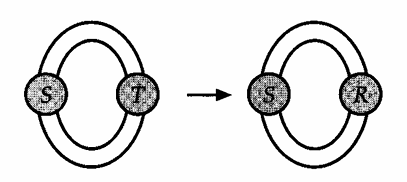
\includegraphics[width=0.75\linewidth]{images/substrat.png}
    \label{substrat}
    \cite{adams2004knot}
\end{figure}
\end{column}
\end{columns}
\end{frame}
\begin{frame}
\begin{figure}
    \centering
    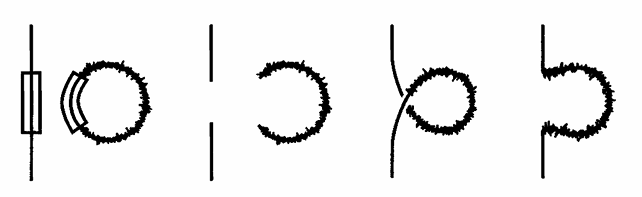
\includegraphics[width=0.6\linewidth]{images/inten.png}
    \label{inten}
\end{figure}
\begin{figure}
    \centering
    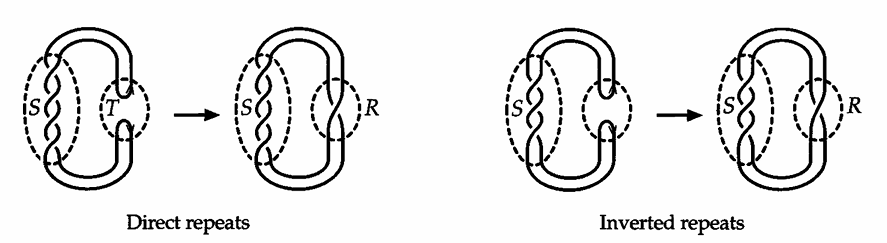
\includegraphics[width=0.75\linewidth]{images/inten2.png}
    \caption{Effects of Int enzyme}
    \label{inten2}
    \cite{adams2004knot}
\end{figure}   
\end{frame}
\begin{frame}{Knots and Chemistry}
\begin{columns}[T]
\begin{column}{.48\textwidth}
\begin{figure}
    \centering
    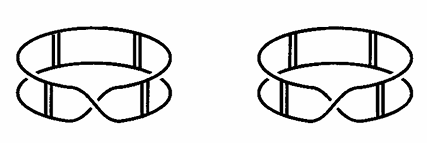
\includegraphics[width=0.8\linewidth]{images/mobius.png}
    \caption{Homeomorphic but not isotopic \centering molecules}
    \label{mobius}
    \cite{adams2004knot}
\end{figure}
\end{column} 
\begin{column}{.48\textwidth}
\begin{figure}
    \centering
    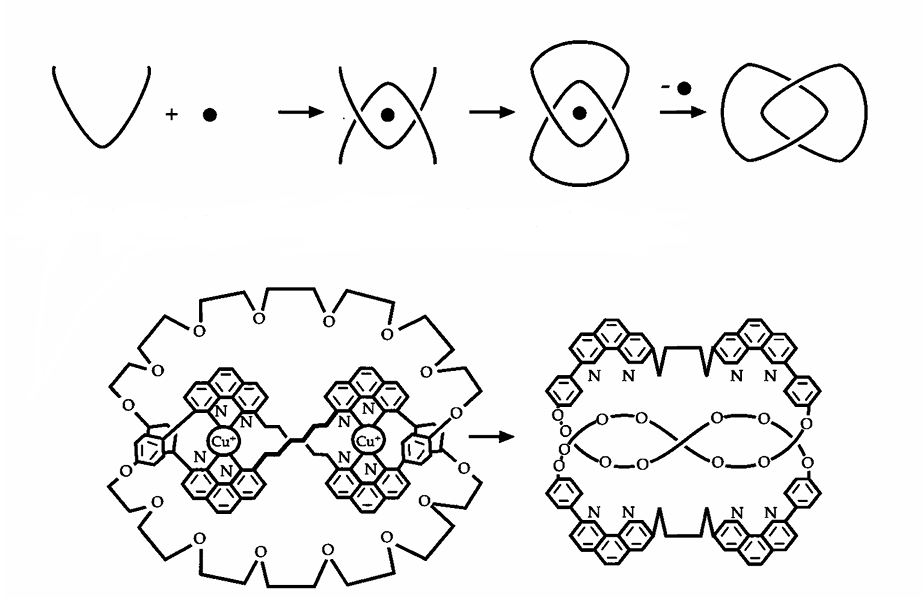
\includegraphics[width=0.9\linewidth]{images/mergedmolecule.png}
    \label{merged}
    \cite{adams2004knot}
\end{figure}
\end{column}
\end{columns}
\end{frame}
\begin{frame}{Knots and Topology}
Poincaré Conjecture: Every three-dimensional topological manifold which is closed, connected, and has trivial fundamental group is homeomorphic to the three-dimensional sphere.
\begin{figure}
    \centering
    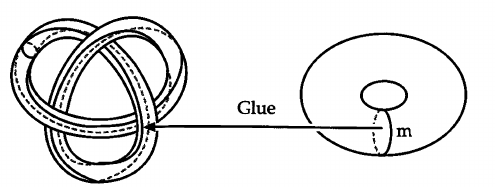
\includegraphics[width=0.5\linewidth]{images/dehn.png}
    \caption{Dehn Surgery}
    \label{dehn}
    \cite{adams2004knot}
\end{figure}
\end{frame}
\begin{frame}{Open Problems}
    \begin{itemize}
        \item Could there be a constant c such that for any knot K and for any two projections P 1 and P2 of K, each with no more than n crossings, one can get from one projection to the other by Reidemeister moves without ever having more than n + c crossings at any intermediate stage?
        \item Find all of the 14-crossing prime knots.
        \item Show that the number of distinct prime (n + 1)-crossing knots is
greater than the number of distinct prime n-crossing knots, for each
positive integer n.
        \item Is it true that a knot with
unknotting number n cannot be a composite knot with n + 1 factor
knots?
\item Show that the crossing number of a composite knot is the sum of the
crossing numbers of the factor knots, that is, $c(K_1#K_2) = c(K_1) + c(K_2)$
    \end{itemize}
    \cite{adams2004knot}
\end{frame}